\documentclass{acm_proc_article-sp}
\usepackage{minted}
\usepackage{hyperref}
\usepackage{ngerman}
\usepackage{graphics}
\usepackage{float}
\usepackage{colortbl}
\usepackage{amsmath}
\usepackage{breakurl}
\hypersetup{
    pdftitle={Complex Event Processing am Beispiel von Esper },
    pdfauthor={Martin Steinbach},
    pdfkeywords={Seminar, Rostock, WiSe 2018, 2018},
    pdfsubject={Seminar Event Driven Programming},
    pdfcreator={Martin Steinbach},
    citecolor=blue,
    hypertexnames=false,
    %linktocpage,
    pdfpagelabels,
    plainpages=false,
    backref,
    urlcolor=blue,
    menucolor=red,
    linkcolor=black,
    colorlinks=true,
    bookmarksnumbered,
    %pdffitwindow
}
%\hyphenation{
 
%}

\usemintedstyle{}


\definecolor{shadecolor}{gray}{.95}
\hyphenation{pattern}


\begin{document}


\title{Complex Event Processing am Beispiel von Esper}
\numberofauthors{1} 
\author{
\alignauthor
Martin Steinbach\vspace{0.1cm}\\
       \affaddr{Institut für Informatik}\\
       \affaddr{Universität Rostock}\\
       %\affaddr{Rostock, Deustchland}\\
       \email{\footnotesize martin.steinbach@uni-rostock.de}}




\maketitle

\begin{abstract}
\vspace{0.1cm}
Die Verarbeitung von Ereignissen tritt zunehmend in den Vordergrund. Das ist nicht 
zuletzt der günstigen Sensortechnik und der Überwachung von Prozessen oder Märkten 
geschuldet. In all diesen Anwendungsgebieten werden Ereignisse erzeugt und das oft in 
einem Ausmaß, dass eine Speicherung unmöglich wird, oder der Informationsgehalt der 
Ereignisse schon nah kurzer Zeit sinkt. \textit{Complex Event Processing} bietet eine 
Möglichkeit diese Ereignisse annähernd in Echtzeit zu analysieren und zu korrelieren um 
neues Wissen zu erzeugen und auf Basis dieser neuen Erkenntnisse zu reagieren. Die 
vorliegende Arbeit bietet eine kompakte Einführung in das Thema \textit{Complex Event 
Processing} und deren zugrunde liegenden Anfragesystematiken. Hauptaugenmerk liegt jedoch 
in der beispielhaften Veranschaulichung dieser Systematiken anhand der Anfragesprache 
\textit{EPL} der \textit{CEP}-Software Esper.

\end{abstract}

%\terms{Theory}

\keywords{EDA, CEP, EPL, Esper} % NOT required for Proceedings

\section{Einleitung}
\vspace{0.1cm}
Jede Aktion in der IT-gestützten Welt erzeugt 
Informationen in Form von Daten. Dabei spielt es keine Rolle ob ein Verweis in einem 
sozialen Netzwerk verwendet wird, ob ein Sensor einen Messwert meldet, oder jemand eine 
Aktie kauft. Betrachtet man diese Daten, scheint der Informationsgehalt gering und die 
Datenmenge überschaubar. Aus diesen Grund lässt sich aus diesen Einzelinformationen kaum 
eine nutzbringende Auskunft für ein Gesamtsystem konstruieren. In der Praxis relevante
Fragestellungen wären zum Beispiel: Wie oft wird ein Verweis innerhalb einer Zeitspanne 
ausgelöst und zu welcher Tageszeit hauptsächlich? Wie viele Messwerte eines Sensors 
werden benötigt um konkrete Aussagen zu einem Messobjekt machen zu können? Wann und 
welche Menge an Aktien eines Unternehmens werden über einen Zeitraum erworben, 
beziehungsweise verkauft?\\
Um diese exemplarischen Fragen zu beantworten steigt die Anzahl der benötigten Daten sehr 
schnell an und eine Verarbeitung mit anschließender Analyse der Daten bedarf wesentlich 
mehr Aufwand und Zeit. Möchte man zudem nicht nur historische Daten analysieren, sondern 
möglichst ohne Zeitverzögerung eine Antwort auf aktuell erhobene Daten erhalten, dann 
bietet sich die Technologie \textit{Complex Event Processing (CEP)} an. Mithilfe der von 
\textit{CEP} angebotenen Verfahren lassen sich riesige und aktuellste Datenmengen nahezu 
direkt verarbeiten. Im Gegensatz zu Datenbankmanagementsystemen, in denen man auf einer 
endlichen Menge an Daten operiert, existieren auch für \textit{CEP} fertige 
Softwarelösungen zur systematischen Analyse von massiven Datenströmen. Eine dieser 
sogenannten \textit{CEP-Engines} ist Esper, laut \cite{fraunhofer} besitzt Esper eine 
sehr große Verbreitung, wird im kommerziellen Umfeld von Namhaften Unternehmen 
verwendet und weist keinen Fokus auf eine spezielle Art der Verwendung auf. Esper ist 
freie Software\footnote{General Public License v2} und steht damit der Gemeinheit für 
jeden 
Zweck zur Verfügung.\\
Neben der Erklärung der Esper-eigenen Abfragesprache \textit{EPL}, werden zuvor die 
Grundlagen von \textit{Complex Event Processing} erläutert. Darunter fällt die Klärung 
essentieller Begriffe, eine Einordnung von \text{CEP} und die Erklärung von 
Abfragesystematiken.

%
% Hauptteil
%

\section{CEP am Beispiel von Esper}
\vspace{0.1cm}

Um die Mechanismen der Anfragesprache \textit{EPL} zu verstehen, muss zuvor im Abschnitt 
\ref{kap:einordnung} die Frage 
geklärt werden wie sich \textit{Complex Event Processing} eigentlich charakterisieren 
lässt und wie es in das System der Datenverarbeitung eingegliedert werden kann. Darüber 
hinaus werden in diesem Abschnitt auch grundlegende Begriffe des \textit{CEP}-Kontext 
geklärt. Abschnitt \ref{kap:anfragesprachen} befasst sich mit allgemein gültigen Aussagen 
zu Anfragesprachen und stellt geläufige Anfragealgebren vor. Der sich anschließende 
Abschnitt \ref{kap:esper} stellt die Funktionsweise von Esper aus Sicht eines Nutzers dar 
und listet in einem kurzen Quellcodefragment, das Vorgehen um Esper in Betrieb nehmen zu 
können. Der ausführlichste Teil, Abschnitt \ref{kap:epl}, zeigt beispielhaft anhand eines 
gegebenem Ereignisstromes, wie sich die Theorie der vorherigen Abschnitte in 
\textit{EPL} realisieren lässt.


\subsection{Einordnung von CEP}\label{kap:einordnung}
\vspace{0.1cm}
\textit{CEP} kann als Bestandteil von \textit{Event-Driven Architecture (EDA)} verstanden 
werden. \textit{EDA} unterscheidet sich als Architekturstil 
grundlegend von anderen Stilen, so findet in \textit{EDA} keine schrittweise Abarbeitung 
von vorher definierten Anweisungen statt um Daten zu verarbeiten. Wie in \cite{glossary} 
beschrieben, existieren stattdessen ereignisgesteuerte Komponenten, deren Interaktion 
untereinander ebenfalls über Ereignisse erfolgt. Damit ist der Begriff des Ereignisses 
ein elementarer und wird in Abschnitt \ref{begriffsbestimmung} ausführlich behandelt. 
\textit{CEP} kann wiederum als Komponente in einem \textit{EDA}-System zum Einsatz 
kommen, wie in Abbildung \ref{img:eda-struktur} aus \cite{bruns}.

\begin{figure}[H]
    \centering
    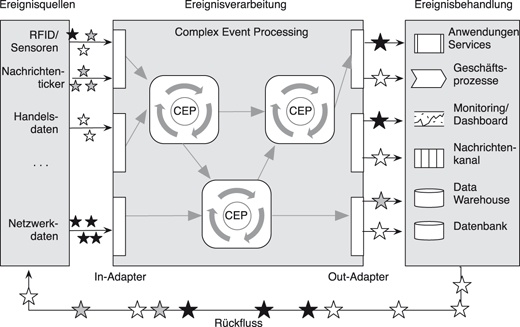
\includegraphics[width=\linewidth]{img/eda-struktur-bruns.jpg}
    \caption{\textit{EDA}-Struktur}
    \label{img:eda-struktur}
\end{figure}

\textit{CEP} ist in erste Linie als Sammelbezeichnung für verschiedene Paradigmen und 
Techniken für die Analyse und Verarbeitung von Ereignissen zu verstehen. Ziel ist es 
Wissen aus einer kontinuierlich nachströmenden Menge an Daten in Form von Ereignissen zu 
generieren. Dies geschieht zum Beispiel durch Korrelation oder Gruppierung von 
Ereignissen nach vorher definierten Regeln. Dabei kann eine Vielzahl von 
Ereignisquellen (Abbildung \ref{img:eda-struktur}) existieren, welche fortlaufend neue 
Ereignisse generieren. Trifft eine Regel auf eine Menge an Ereignissen zu, so wird daraus 
ein komplexes Ereignis (\cite{glossary}) generiert, welches abermals als atomares 
Ereignis für eine weitere 
\textit{CEP}-Instanz dienen kann. Ein komplexes Ereignis wird auch verwendet
um verschiedenartige Meldungen zu generieren, Prozesse zu initiieren oder um als 
Grundlage 
für Visualisierungen zu dienen. In \cite{bruns} wird ein Grundzyklus für 
ereignisgesteuerte Systeme identifiziert (Abbildung \ref{img:cep-zyklus}), der aus den 
drei Schritten Erkennen, Reagieren und Verarbeiten besteht.

\begin{figure}[H]
    \centering
    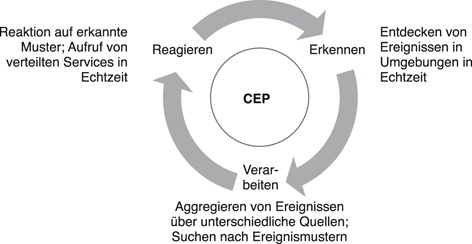
\includegraphics[width=\linewidth]{img/cep-zyklus-bruns.jpg}
    \caption{\textit{CEP}-Zyklus}
    \label{img:cep-zyklus}
\end{figure}

Den Beginn stellt dabei das \emph{Erkennen} dar, relevante Informationen (zum Beispiel 
Messwerte) werden ohne Verzögerung als Ereignisse interpretiert. Während der 
\emph{Verarbeitung} wird die Mustererkennung auf einen oder mehreren Ereignisströmen 
durchgeführt. Sobald Muster erkannt werden, \emph{Reagiert} man mit Meldungen oder mit 
der Generierung komplexer Ereignisse.\\
Laut \cite{eckert} gibt es zwei grundlegende Arten um 
komplexe Ereignisse zu identifizieren. Entweder über bereits bekannte Muster, die durch 
Regeln in Ereignisanfragesprachen formuliert werden können, oder über unbekannte Muster. 
Letztere benötigt allerdings Technologien wie \textit{MachineLearning} und 
\textit{DataMining}, daher wird in diesem Papier nicht darauf eingegangen.

\subsubsection{Begriffsbestimmungen}\label{begriffsbestimmung}
\vspace{0.1cm}
\textbf{\textit{Datenströme/Ereignisströme}}
sind kontinuierliche, kleinteilige Datensätze in der 
zeitlichen Reihenfolge ihres Auftretens oder ihrer Messung. Die Daten weisen eine geringe 
Komplexität auf und beziehen sich nur auf ein Datum (zum Beispiel den Messwert eines 
Sensors oder den Kurs eines Wertpapiers.). Die Ströme sind sind endlos und meist 
hochfrequent und massiv, daher können die Daten nicht persistent gespeichert werden.\\
Jeder Datensatz in einem Datenstrom bildet ein eigenes 
\textbf{\textit{Ereignisse}}. Im 
Allgemeinen kann laut \cite{glossary} ein Ereignis alles sein was eintreten kann, wie zum 
Beispiel ein Erdbeben, eine Finanztransaktion, das Betätigen einer Taste oder die 
Oktoberrevolution. Im speziellen ist ein Ereignis ein aufbereiteter Datensatz, welcher 
die Informationen eines Ereignisses beinhaltet und für die rechnergestützte Verarbeitung 
angepasst ist. Dazu ist es notwendig, dass zum Informationsgehalt des Ereignisses (den 
Kontextinformationen) auch eindeutige und strukturierte Metadaten erfasst werden. 
Exemplarisch 
kann ein Ereignis folgendermaßen aufgebaut sein (\cite{hedtstuck}):

\begin{table}[ht]
    \caption{Ereignisaufbau}
    \label{table:ereignis}\vspace{0.2cm}
    \centering{
        \renewcommand{\arraystretch}{1.3}
        \begin{tabular}{|l|c|}
            \hline
            \multicolumn{2}{|l|}{\cellcolor{shadecolor}\textbf{Metadaten}}\\
            \hline
            Ereignistyp\hspace{0.5cm} &   \texttt{Kursänderung}\\ 
            \hline
            Ereignisquelle\hspace{0.5cm} &   \texttt{Frankfurt}\\ 
            \hline 
            Zeitstempel &   \texttt{2018-11-21 22:14:00}\\
            \hline
            ID          &   \texttt{98127634}\\  
            \hline
            \multicolumn{2}{|l|}{\cellcolor{shadecolor}\textbf{Kontextinformation}}\\     
            \hline
            \multicolumn{2}{|l|}{\texttt{Name: ACME GmbH}}\\
            \multicolumn{2}{|l|}{\texttt{Einkaufkurs: 32.5}}\\
            \multicolumn{2}{|l|}{\texttt{Letzter Kurs: 40.8}}\\
            \multicolumn{2}{|l|}{\texttt{Differenzbetrag: 5.7}}\\
            \multicolumn{2}{|l|}{\texttt{Aktueller Kurs: 42.1}}\\
            \hline
        \end{tabular} 
    }
\end{table}
Wobei die Felder \textit{Ereignistyp} und \textit{Ereignisquelle} nach \cite{bruns} 
optional sind. Wie man an den Metainformationen erkennen kann, stehen alle Ereignisse in 
impliziter Beziehung zueinander.\\
Im Verarbeitungsschritt (Abbildung \ref{img:cep-zyklus}) werden Beziehungen zwischen 
Ereignissen gesucht, diese werden durch \textbf{\textit{Ereignismuster}} beschrieben. Die 
Mustererkennung wird nur über einem bestimmtes Zeitintervall des Ereignisstromes 
ausgeführt und durch Ereignisanfragesprachen definiert. In \cite{bruns} werden drei Arten 
von Ereignismustern unterschieden. Können Muster ausschließlich durch boolesche 
Operatoren der Aussagelogik festgelegt werden, so fallen sie in die Kategorie der 
\textit{einfachen Ereignismuster}. Werden hingegen speziellere Operatoren nötig, um zum 
Beispiel die Reihenfolge oder Zeitfenster in den Ereignisse auftreten auszudrücken, 
gehören sie zur Kategorie der \textit{komplexen Ereignismuster}. Zur Kategorie der 
\textit{Abstrakten Ereignismuster} gehören die Muster, welche aus einem bereits erkannten 
Muster komplexe Ereignisse erzeugt um diese auf einer höheren Abstraktionsebene wieder 
zur Verfügung zu stellen.\\
Ein \textbf{\textit{Komplexes Ereignis}} ist eine Menge von Ereignissen, die durch ein 
Ereignismuster beschrieben sind.\\\label{begriff-ereignisregel}
\textbf{\textit{Ereignisregeln}} sind die syntaktische Abstraktion von Ereignismustern 
und werden mithilfe einer \textbf{\textit{Anfragesprache}} erstellt, laut \cite{bruns} 
existieren für diese 
Sprachen kein einheitlicher Standard. Daher existiert eine Fülle an Sprachen, die aber 
alle einige Eigenschaften Teilen. So bestehen alle in einer Anfragesprache formulierten 
Regeln aus einer Prämisse und einem Aktionsteil, wenn das Muster, Beziehungsweise die 
Bedingung in der Prämisse erfüllt ist, wird der Aktionsteil ausgeführt. Anfragesprachen 
sind grundsätzlich deklarativ, man beschreibt also ein Modell und muss keine Verfahren 
zur Mustererkennung implementieren. In \cite{eckert} werden auch reaktive Regeln erwähnt, 
diese Regeln definieren, wie auf komplexe Ereignisse reagiert werden soll.

\subsubsection{Beispielanwendungen}
\vspace{0.1cm}

\textit{CEP} kommt überall dort zum Einsatz wo Daten möglichst in Echtzeit analysiert 
werden sollen um Erkenntnisgewinn zu erlangen. Die Finanzbranche ist sicherlich einer der 
größten Sektoren in dem \texttt{CEP} zum Einsatz kommt. Dabei muss es sich nicht um 
zeitnahe Analysen der Marktsituation oder automatisierten Handel handeln, auch die 
Erkennung von 
Kreditkartenmissbrauch wird mittels \textit{CEP} automatisiert. \textit{CEP} wird auch 
zur Überwachung von Industrieanlagen und im Automobilbereich eingesetzt um schnell die 
Informationen einer Vielzahl von Sensoren zu interpretieren. Auch das CERN wäre ohne 
\textit{CEP} nicht in der Lage die Daten der verschiedenen Detektoren am LHC auszuwerten, 
denn eine Speicherung der Daten zur späteren Analyse ist aufgrund der Menge unmöglich.\\
Zu Erwähnen ist auch die \textit{DEBS}-Konferenz\footnote{Ditributet Event Based Systems: 
\url{http://debs.org/debs-conferences/}} und deren \textit{Grand Challenges}, ein seit 
2010, jährlich veröffentlichtes Problem was auf Basis einer riesigen Datenmenge zu lösen 
ist.


%
% Anfragesprachen
%
\subsection{Anfragesprachen}\label{kap:anfragesprachen}
\vspace{0.1cm}
Mithilfe von Ereignisanfragesprachen lassen sich Daten aus einer Ereignisfolge, eine 
endliche Menge an Ereignissen innerhalb des endlosen Ereignisstromes, extrahieren, 
verdichten, zeitliche zusammenhänge herstellen und Aktionen festlegen.

\subsubsection{Definition von Ereignisregeln}\label{kap:ereignisregeln}
\vspace{0.1cm}
In diesem Abschnitt wird eine Übersicht über die zur Verfügung stehenden Mengenalgebren 
in Anfragesprachen gegeben, dabei wird sich auf das Vorgehen in \cite{bruns} berufen.\\
Seien $A,B,C$ Ereignistypen und $a,b,c$ zugehörige Ereignisinstanzen, wobei gilt 
$a \in A$, $b \in B$ und $c \in C$. Eine Ereignisfolge wird durch $a_1a_2a_3b_1c_1b_21_4$
beschrieben.\\
Jede Ereignisalgebra enthält spezielle Operatoren, die auf Ereignisfolgen angewendet 
werden können und dabei z.B. zeitliche, kausale oder fachliche Zusammenhänge zwischen 
Ereignissen beschreiben. In \textbf{\textit{ereignistypbasierten Mustern}} legt der 
Sequenzoperator die zeitliche Reihenfolge des Auftretens von Ereignistypen fest. Zum 
Beispiel $A \rightarrow B$. Diese Regel akzeptiert die Ereignisfolge $c_1a_1a_2c_2b_1$. 
Des Weiteren existieren die boolesche Operatoren $\land , \lor$, die keine Reihenfolge 
des Auftretens beschreiben, da das Kommutativgesetz gilt: $A \circ B = B \circ A, \circ 
\in {\lor,\land}$. Ebenso existiert die Negation: $\neg A$. Die Kombination dieser 
Operatoren ermöglicht es komplexe Muster in Ereignisfolgen zu erkennen.\\
Eine weitere Algebra, welche von Anfragesprachen implementiert wird, ist die Algebra über 
\textbf{\textit{Kontextbedingungen}}. Mithilfe dieser Algebra ist es möglich direkt 
auf Attribute der Ereignisinstanzen über den $.$-Operator zugreifen zu können. Damit 
besteht die Möglichkeit die Attribute in Relation zu setzen Rechenvorschriften zu 
definieren. Zur Verfügung stehen dabei die numerischen Operatoren und 
Vergleichsoperatoren, aber auch Operatoren für Zeichenketten sind denkbar, oder gesondert 
definierte Methoden. Um in dieser Algebra verschiedene Entitäten von Ereignistypen zu 
betrachten, ist ein Operator zur Namenssubstitution vorhanden. Dieser Operator weist 
einem Ereignis eines Ereignistyps einen neuen Namen zu. Dieser binäre Operator könnte zum 
Beispiel $AS$ lauten. Das folgende Muster würde demnach die Werte des Attributes 
$humidity$ von einem Ereignis mit dem Ereignistyp $A$ mit einem Ereignis vom 
nachfolgenden Ereignistyp $B$ auf Gleichheit prüfen.
$$((A\, AS\, a)) \rightarrow (B\, AS\, b)) \land (a.humidity = b.humidity)$$
Aufgrund des endlosen Ereignisstromes, können die zuvor beschriebenen Muster nicht auf 
die ganze Menge der Ereignisse angewendet werden, da diese weder gespeichert werden 
können, oder nach kurzer Zeit schon nicht mehr von Interesse sind. Daher kommen 
sogenannte \textbf{\textit{sliding windows}} zum Einsatz. Diese erlauben es, nur einen 
gewisses Segment des Ereignisstromes für die Mustererkennung zu betrachten. Dabei werden 
laut \cite{bruns} und \cite{hedtstuck} zwei Fensterarten unterschieden. Das Zeitfenster 
berücksichtigt alle Ereignisse, die in einem zuvor festgelegtem Zeitraum eintreffen. 
Betrachtet man hingegen eine maximale Anzahl an Ereignissen innerhalb eines 
Ereignisstromes, dann spricht man von einem Längenfenster. Abbildung 
\ref{img:sliding-windows} aus \cite{drools-slide} verdeutlicht diesen Mechanismus. Dabei 
können die grauen Quader als beliebige Ereignisse oder als Ereignisse die einem 
Ereignismuster entsprechen verstanden werden.

\begin{figure}[H]
    \centering
    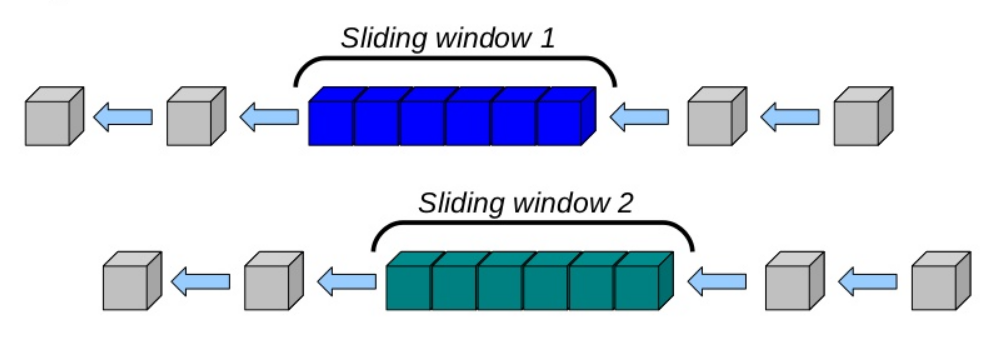
\includegraphics[width=\linewidth]{img/sliding-windows.png}
    \caption{sliding windows}
    \label{img:sliding-windows}
\end{figure}

Eine beispielhafte Ereignisregel mithilfe von sliding windows könnte folgendermaßen 
aussehen:
$$(A \rightarrow B)[win:time:5min] \rightarrow C$$
Dieses Muster ist erfolgreich, wenn innerhalb eines fünf minütigen Zeitfensters ein 
Ereignis des Ereignistyps B auf ein Ereignis des Ereignistyps A folgt und anschließend 
(zeitunabhängig) ein Ereignis vom Ereignistyp C eintritt.\\
Da es möglich ist mehrere Fensterinstanzen auf einen oder mehrere Ereignisströme parallel 
anzuwenden, kann mithilfe eines \textbf{Verschiebefaktors}\label{kap:verschiebefaktor}, 
wie er in \cite{hedtstuck} beschrieben 
ist, die Schnittmenge zweier aufeinanderfolgender Fenster angegeben werden. Dabei 
unterscheidet \cite{hedtstuck} nochmals in die \textit{Rolling Windows}, bei denen der 
Verschiebefaktor kleiner als die Länge des Fensters ist und zwei aufeinanderfolgende 
Fenster somit eine Schnittmenge besitzen und \textit{Tumbling Windows}, deren 
Verschiebefaktor größer oder gleich der Fensterlänge ist. Aufeinanderfolgende 
\textit{Tumbling Windows} sind zueinander Disjunkt und ist der Verschiebefaktor größer 
als die Fensterlänge, befinden sich zwischen ihnen nicht betrachtete Ereignisse. 
Abbildung \ref{img:factors} aus \cite{hedtstuck} zeigt den Einfluss des 
Verschiebefaktors auf aufeinanderfolgender Fensterinstanzen.

\begin{figure}[H]
    \centering
    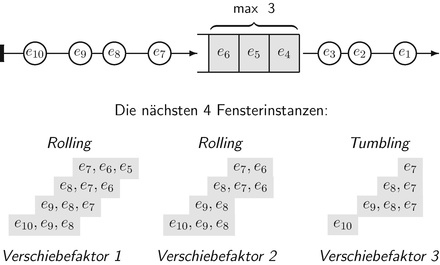
\includegraphics[width=\linewidth]{img/factor-hedstuck}
    \caption{Verschiebefaktor}
    \label{img:factors}
\end{figure}

\subsubsection{Definition von Aktionen}
\vspace{0.1cm}
Wird ein Ereignismuster erkannt und ist damit die Prämisse einer Ereignisregel erfüllt, 
muss eine Aktion ausgeführt werden. Eine Aktion kann die Erstellung neuer Ereignisse 
sein, oder das Ausführen von Diensten, beziehungsweise Versenden von Meldungen.\\
Werden neue Ereignisse Erzeugt, so ist von der Ereignistransformation die Rede. In 
\cite{bruns} wird zwischen zwei Transformationen unterschieden. Den Transformationen, die 
keine Informationen zu einer transformierten Ereignisfolge hinzufügen und diejenigen, die 
dies tun. So kann im einfachsten Fall ein Ereignis eines gewissen Ereignistyps zu einem 
anderen Ereignistyp zugeordnet werden. Aktionen in Anfragesprachen erlauben auch die 
Filterung von Ereignissen. Mit einer gefilterten Menge an relevanten Ereignissen kann 
eine Leistungssteigerung der Musterkennung erfolgen. Zudem lässt sich eine Menge an 
Ereignissen zu einem neuen Ereignis zusammenfassen.\\
Darüber hinaus kann auch der Informationsgehalt von Ereignissen verändert werden, indem 
man Daten hinzufügt oder entfernt, zum Beispiel im Zuge einer Normalisierung eines 
Datenformats. Das generieren von komplexen Ereignissen erfolgt über Korrelation mehrerer 
einfacher Ereignisse, aus denen sich domänenspezifisches Wissen ableiten lässt. Als 
Beispiel soll die Erkennung einer \textit{BruteForce}-Attacke dienen:
\begin{align*}
&CONDITION:\\
&\quad (FailedLoginAttempt\, AS\, f)[win:time:5min]\\
&\quad \land\quad f.SourceIP\, =\, ''::1'' \\
&\quad \land\quad f.sum(count)\, AS\, FailCounter\\
&\quad \land\quad FaileCounter >= 10\\
&ACTION:\\
&\quad create \quad BruteForceAttack(SourceIP = f.SourceIP,\\
&\quad \quad Time=timestamp())
\end{align*}

%
% ESPER
%
\subsection{Esper}\label{kap:esper} 
\vspace{0.1cm}

Esper ist eine \textit{Complex Event Processing Engine} und stellt eine Laufzeitumgebung 
und einen Compiler für die eigene Ereignisanfragesprache \textit{Event Processing 
Language (EPL)} zur Verfügung. Der Compiler Übersetzt \textit{EPL} in Bytecode für die 
\textit{Java Virtual Machine}. Esper ist ebenfalls in der Programmiersprache Java 
implementiert, mit Nesper existiert allerdings auch eine Implementierung in C\#. Da nicht 
auf einer endlichen Menge an Daten nach Mustern gesucht wird, lässt sich Esper eher als 
eine invertierte Datenbank verstehen. Als erstes teilt man dem Compiler mithilfe einer 
zuvor erstellten Konfiguration das Event-Schema mit, um ihm anschließend ein 
EPL-Statement zur Übersetzung zur Verfügung zu stellen (Abbildung \ref{java:01}). 

\begin{figure}[h]    
\begin{minted}[mathescape,bgcolor=shadecolor]{java}
EPCompiler c = EPCompilerProvider.getCompiler();
Configuration conf = new Configuration();
conf.getCommon().addEventType(PersonEvent.class);

CompilerArguments cargs = 
    new CompilerArguments(conf);
EPCompiled epCompiled;
epCompiled = c.compile("@name('statement')
    select name, age from PersonEvent
    where (age/5) > 5", cargs);
\end{minted}
\caption{Initialisierung des Compilers}
\label{java:01}
\end{figure}

Die Laufzeitumgebung verwendet dann das zuvor übersetzte Statement und wendet es auf 
einen Ereignisstrom an. Ereignisse sind in diesem Fall Objektinstanzen der Klasse 
PersonEvent. Ein \textit{Listener} kann die zutreffenden Resultate verarbeiten. In 
diesem Beispiel (Abbildung \ref{java:02}) aus \cite{esper-reference} werden die 
Ereignisparameter \textit{name} und \textit{age} ausgegeben.

\begin{figure}[h]    
\begin{minted}[mathescape,bgcolor=shadecolor]{java}
EPRuntime rt =
    EPRuntimeProvider.getDefaultRuntime(conf);
    
EPDeployment deployment;
deployment =
    rt.getDeploymentService().deploy(epCompiled);
    
EPStatement statement =         
    rt.getDeploymentService().getStatement(
        deployment.getDeploymentId(),"statement");
        
statement.addListener(new UpdateListener() {
public void update(EventBean[] newData,
    EventBean[] oldData, EPStatement statement,
    EPRuntime rt) {
    
    String name = (String) newData[0].get("name");
    int age = (int) newData[0].get("age");
    System.out.println(
        String.format("Name: %s,
            Age: %d",name, age));
}});
\end{minted}
    \caption{Initialisierung der Laufzeitumgebung}
    \label{java:02}
\end{figure}

Um an die Esper-Laufzeitumgebung Ereignisse zu senden, müssen neue Ereignisinstanzen 
Erzeugt werden und an die Laufzeitumgebung gesendet werden, wie in Abbildung \ref{java:03}
gezeigt

\begin{figure}[h]    
\begin{minted}[mathescape,bgcolor=shadecolor]{java}
for (int i = 0; i <= 100; i++) {
runtime.getEventService().sendEventBean(
    new PersonEvent("Peter", i), "PersonEvent");
}
\end{minted}
\caption{Senden von Ereignissen}
\label{java:03}
\end{figure}

\subsection{Die Anfragesprache EPL}\label{kap:epl}
\vspace{0.1cm}
Die \textit{Event Processing Language} von Esper ist stark an \textit{SQL} angelehnt, 
bietet aber Erweiterungen für die Verarbeitung von Ereignissen in einem endlosen 
Ereignisstrom. Ähnlich wie bei SQL ist ein statement folgendermaßen aufgebaut:

\texttt{select DATENAUSWAHL from EREIGNISSTROM where FILTER}

Um Anfragen an einen Ereignisstrom zu validieren, bietet der Entwickler von Esper, 
EsperTech Inc., das Werkezug 
\textit{EPL}-Online\footnote{\url{http://esper-epl-tryout.appspot.com/epltryout/mainform.html}}
an. Basierend auf den 
Voreinstellungen in \textit{EPL}-Online werden die nachfolgenden Beispielanfragen an den 
Ereignisstrom \texttt{StockTick} gerichtet. Der Zugehörige Ereignistyp wurde zuvor durch 
das folgende EPL-statement definiert. Die neu erzeugten Ereignisse werden als 
\textit{callbacks} durch einen \textit{Listener} entgegengenommen und sind als Ausgabe 
verfügbar.

\texttt{create schema StockTick(symbol string, price double);}

Die verwendeten Datentypen sind stark an die primitiven Datentypen der Programmiersprache 
Java angelehnt (\texttt{boolean, integer, long, double, float, byte}). Es existiert aber 
auch der Datentyp \texttt{string}, für die Speicherung von unbegrenzt großen 
Zeichenketten.

Für die Beispiele wird folgender Ereignisstrom verwendet.

\begin{verbatim}
StockTick={symbol='YHOO', price=65}
StockTick={symbol='IBM', price=141}
t=t.plus(2 seconds)
StockTick={symbol='IBM', price=142}
StockTick={symbol='YHOO', price=62}
t=t.plus(2 seconds)
StockTick={symbol='IBM', price=146}
StockTick={symbol='YHOO', price=63}
t=t.plus(2 seconds)
StockTick={symbol='YHOO', price=64}
StockTick={symbol='IBM', price=147}
t=t.plus(6 seconds)
\end{verbatim}

Die Variable \texttt{t} symbolisiert dabei die vergangene Zeit zwischen dem Eintreten von 
Ereignissen. Dabei sind \texttt{t = t+2000} und \texttt{t=t.plus(2 seconds)} äquivalente 
Ausdrücke. 

Das einfachste Muster, dass mithilfe von EPL beschrieben werden kann, ist die Filterung 
aller Ereignisse.

\texttt{select * from StockTick();}

Einfache Bedingungen lassen sich mit \texttt{where} realisieren. Zusätzlich lässt Esper 
noch eine weitere Schreibweise für Bedingungen zu, diese zweite Schreibweise ist 
äquivalent zur Ersten, erhöht jedoch die Lesbarkeit in den später behandelten 
ereignistypbasierenden Mustern.

\texttt{select * from StockTick() where price > 100;}\\
\texttt{select * from StockTick(price > 100);}

Eine Aggregation über alle Events kann mittels vordefinierter Funktionen erfolgen. EPL 
stehen neben den einfachen Funktionen wie \texttt{avg(), count(), sum()} auch 
statistische Methoden zur Verfügung (siehe Tabelle 10.5 in \cite{esper-reference}).

Die nächste Anfrage zählt die Anzahl aller Ereignisse und bildet den Durchschnitt über 
alle Kurspreise der IBM-Aktie.

\texttt{select  count(*),avg(price) from StockTick()\\where symbol='IBM'}

Die zuvor gezeigten Beispiele eignen sich nicht zur Anfrage auf einen endlosen 
Ereignisstrom, da alle Ereignisse angefragt werden. Ein endgültiges Ergebnis würde ein 
Ende des Ereignisstromes voraussetzen, daher finden im Rahmen von \textit{CEP} die in 
Kapitel \ref{kap:ereignisregeln} beschriebenen Fenster Verwendung. Die anschließende 
EPL-Anfrage setzt ein auf Zeit basierendes \textit{sliding window} ein und berechnet den 
Durchschnittspreis der IBM-Aktie der letzten 6 Sekunden:

\texttt{select  avg(price) from StockTick().win:time(6 sec)\\where symbol='IBM'}

Da es sich hierbei um ein normales Zeitfenster ohne expliziten Verschiebefaktor handelt 
(siehe auch Abschnitt \ref{kap:verschiebefaktor}), werden insgesamt 7 Ergebnisse 
ausgegeben. Trifft ein Muster auf ein Ereignis zu, so bekommt dieses Ereignis eine 
Gültigkeitsdauer zugeordnet, es ist damit in das Fenster aufgenommen wurden. Läuft die 
Gültigkeitsdauer ab, so wird das Ereignis aus dem Fenster entfernt. Tabelle 
\ref{table:ereignis} soll die Funktion der einfachen Zeitfenster in Esper verdeutlichen. 
Dabei wird sich auf den oben eingeführten Ereignisstrom und die letzte Anfrage bezogen.

\begin{table}[ht]
    \caption{Fenster ohne Verschiebefaktor}
    \label{table:ereignis}\vspace{0.2cm}
    \centering{
        \renewcommand{\arraystretch}{1.3}
        \begin{tabular}{|c|c|c|c|l|}
            \hline
            \cellcolor{shadecolor}Fenster   &\cellcolor{shadecolor} 2 Sek.    
            &\cellcolor{shadecolor} 4 Sek.    &\cellcolor{shadecolor} 6 Sek. & 
            \cellcolor{shadecolor}callback\\  
            \hline
            1   &       &        &\textbf{141},65         &   141\\
            2   &       &\textbf{141},65   &\textbf{142},64         &   141.5\\
            3   &\textbf{141},65  &\textbf{142},62   &\textbf{146},63         &   143\\
            4   &\textbf{142},62  &\textbf{146},63   &              &   144\\
            5   &\textbf{142},62  &\textbf{146},63   &\textbf{147},64         &   145\\
            6   &\textbf{146},63  &\textbf{147},64   &              &   146.5\\
            7   &\textbf{147},64  &        &              &   147\\
        \hline   
        \end{tabular} 
    }
\end{table}

Da dieses Vorgehen wenig Intuitiv erscheint existieren in EPL auch Längen- und 
Zeitfenster mit einem fixen Verschiebefaktor. Die sogenannten \texttt{batch}-Fenster sind 
\textit{Tumbling Windows}, deren Verschiebefaktor der Länge des jeweiligen Fensters 
entspricht. Die gleiche Anfrage mithilfe eines \texttt{batch}-Fensters verhält sich 
folgendermaßen.

\texttt{select  avg(price) from StockTick().win:time\_batch(6 sec)where symbol='IBM'}

\begin{table}[ht]
    \caption{\texttt{batch}-Fenster}
    \label{table:ereignis-batch}\vspace{0.2cm}
    \centering{
        \renewcommand{\arraystretch}{1.3}
        \begin{tabular}{|c|c|l|}
            \hline
            \cellcolor{shadecolor}Fenster   &\cellcolor{shadecolor} 6 Sek.& 
            \cellcolor{shadecolor}callback\\  
            \hline
            1   &65, \textbf{141}, \textbf{142}, 62, \textbf{146}, 63 &   143\\
            2   &64,\textbf{147}       &    147\\
            \hline   
        \end{tabular} 
    }
\end{table}

Anfragen mithilfe von einfachen Längenfenstern lassen sich ebenso leicht definieren und 
verhalten sich genauso wie eine Warteschlange. Es werden nur Ereignisse innerhalb des 
Längenfensters betrachtet, die dem Filter hinter der \texttt{where}-Anweisung 
entsprechen. Dabei werden durch Esper immer dann Aktionen ausgelöst, die als sogenannte 
\textit{callbacks} an den \textit{Listener} gesendet werden, wenn ein relevantes Ereignis 
das Fenster betritt oder verlässt. Die Folgende Tabelle \ref{table:warteschlange} 
demonstriert dieses Vorgehen.

\texttt{select avg(price) from StockTick().win:length(4)\\where symbol='IBM'}

\begin{table}[ht]
    \caption{Längenfenster}
    \label{table:warteschlange}\vspace{0.2cm}
    \centering{
        \renewcommand{\arraystretch}{1.3}
        \begin{tabular}{|c|c|c|c|c|l|}
            \hline
            \cellcolor{shadecolor}Fenster   &\cellcolor{shadecolor} 1    
            &\cellcolor{shadecolor} 2    &\cellcolor{shadecolor} 3 & 
            \cellcolor{shadecolor}4 &\cellcolor{shadecolor}callback\\  
            \hline
            1   &65 & & & &- \\
            2   &\textbf{141} &65 & & &141 \\
            3   &\textbf{142} &\textbf{141} &65 & &141.5 \\
            4   &62 &\textbf{142} &\textbf{141} &65 &- \\
            5   &\textbf{146} &62 &\textbf{142} &\textbf{141} &143 \\
            6   &63 &\textbf{146} &62 &\textbf{142} &144 \\
            7   &64 &63 &\textbf{146} &62 &146 \\
            8   &\textbf{147} &64 &63 &\textbf{146} &146.5 \\
            \hline   
        \end{tabular} 
    }
\end{table}

Aufeinanderfolgende \texttt{batch}-Längenfenster überschneiden sich hingegen nicht.

\texttt{select  avg(price) from StockTick().win:length\_batch(4)\\where symbol='IBM'}
\begin{table}[ht]
    \caption{\texttt{batch}-Längenfenster}
    \label{table:warteschlange-batch}\vspace{0.2cm}
    \centering{
        \renewcommand{\arraystretch}{1.3}
        \begin{tabular}{|c|c|c|c|c|l|}
            \hline
            \cellcolor{shadecolor}Fenster   &\cellcolor{shadecolor} 1    
            &\cellcolor{shadecolor} 2    &\cellcolor{shadecolor} 3 & 
            \cellcolor{shadecolor}4 &\cellcolor{shadecolor}callback\\  
            \hline
            1   &65 &\textbf{141} &\textbf{142} &62 &141.5 \\
            2   &\textbf{146} &63 &64 &\textbf{147} &146.5 \\
            \hline   
        \end{tabular} 
    }
\end{table}

Möchte man mehrere Bedingungen an ein Ereignis stellen, können diese mithilfe 
aussagenlogischer Operatoren beschrieben werden. Die sich anschließende Anfrage ermittelt 
aus jeweils vier Datensätzen, diejenige Kursaktualisierung, die IBM betrifft und den Kurs 
unter einen Wert von 144 fallen lässt.

\texttt{select * from StockTick().win:length\_batch(4)\\where symbol='IBM' and 
price < 144}

Um \textbf{ereignistypbasierte Muster} in EPL zu verwenden, wie sie in Sektion 
\ref{kap:ereignisregeln} erwähnt wurden, existiert das Schlüsselwort \texttt{pattern[]}. 
Mit dessen Hilfe kann man Ereignisse auf einem endlosen Datenstrom detektieren, ohne 
Fenster einzusetzen. Als Grundlage für die folgenden Beispiele soll der folgende, 
angepasste Ereignisstrom dienen. Dem Ereignisstrom wurde ein neuer Ereignistyp namens 
\texttt{NewsTick} mit der Definition
\texttt{create schema NewsTick(symbol string, message string);} hinzugefügt.
\begin{verbatim}
StockTick={symbol='YHOO', price=65}
StockTick={symbol='IBM', price=141}
t=t.plus(2 seconds)
StockTick={symbol='IBM', price=142}
StockTick={symbol='YHOO', price=62}
t=t.plus(2 seconds)
StockTick={symbol='IBM', price=146}
NewsTick={symbol="IBM",message="good"}
StockTick={symbol='YHOO', price=63}
t=t.plus(2 seconds)
StockTick={symbol='YHOO', price=64}
StockTick={symbol='IBM', price=147}
t=t.plus(6 seconds)
StockTick={symbol='YHOO', price=71}
StockTick={symbol='IBM', price=150}
NewsTick={symbol="IBM",message="bad"}
t=t.plus(6 seconds)
StockTick={symbol='YHOO', price=77}
StockTick={symbol='IBM', price=107}
\end{verbatim}

Um mit dem \texttt{pattern[]}-Schlüsselwort auf Ereignisströmen zu operieren muss zuvor 
dessen Mechanismus zur Ereignisauswahl geklärt werden. Im Gegensatz zu Fenstern, wo aus 
einer unendlichen Menge eine klar über die Zeit oder Mächtigkeit definierte, endliche 
Untermenge betrachtet wird, kann die  betrachtete Menge mithilfe des 
\texttt{pattern[]}-Mechanismus unterschiedlich groß in Bezug auf Zeit und Mächtigkeit 
sein. Die Handlungsweise hängt stark von der Anfrage ab und wird mit dem Begriff  
\textit{Event Consumption} belegt. Die Verschiedenen Verfahren wurden in 
\cite{adaikkalavan} ausführlich vorgestellt und in \cite{hedtstuck} in Zusammenhang mit 
Esper gebracht. Betrachtet man eine ereignistypbasierte Regel, die zwei Ereignistypen 
mithilfe des schon beschriebenen Sequenzoperators in Kontext setzt 
(\texttt{pattern[A->B]}), dann wird der Ereignistyp A als Initiator und B als Detektor 
bezeichnet. Ein einfaches Beispiel, angewendet auf den neu eingeführten Ereignisstrom, 
lautet folgendermaßen. Dabei soll die Yahoo-Kurskorrektur gefunden werden, die zeitlich 
auf eine IBM-Kurskorrektur folgt.

\texttt{select b from pattern[a=StockTick(symbol='IBM') ->\\ 
b=StockTick(symbol='YHOO')];}

Das einzige Ergebnis dieser Anfrage ist das Detektorereignis 
\texttt{StockTick=\{symbol='YHOO', price=62\}}. Das Initiatorereignis ist die erste 
Auftretende IBM-Kurskorrektur \texttt{StockTick={symbol='IBM', price=141}}. Wird ein 
Initiatorereignis gefunden, startet Esper einen dedizierten \textit{Event Processing 
Agent (EPA)} (siehe \cite{bruns}), der alle eintreffenden Ereignisse in zeitlicher 
Reihenfolge analysiert. Trifft der \textit{EPA} auf das Detektorereignis wurde das Muster 
erkannt und der angefragte Datensatz wird als Rückgabe bereit gestellt. Auch andere 
logische Operatoren dürfen in diesen Anfragen Verwendung finden. Wird statt dem 
Sequenzoperator \texttt{->} die Konjunktion \texttt{and} verwendet, ändert sich das 
Detektorereignis zu \texttt{StockTick=\{symbol='YHOO', price=65\}}, aufgrund der 
Kommutativität dieses Operators.\\
Aus dieser Darstellung heraus ist erkennbar, dass in diesem Beispiel lediglich ein 
\textit{EPA} gestartet wurde. Zudem geht aus dem Ereignisstrom hervor, dass dieses Muster 
noch auf weitere Ereignisse zutreffen könnte. Um Esper anzuweisen zusätzliche 
\textit{EPA} zu starten muss der Operator \texttt{every} eingesetzt werden. Die folgende 
Anfrage verdeutlicht beispielhaft die Anwendung des 
\textit{Unrestricted Consumption Mode} in EPL.

\texttt{select a.price,b,price from\\pattern[every a=StockTick(symbol='IBM') ->\\
every b=StockTick(symbol='YHOO')];}

Im \textit{Unrestricted Consumption Mode} wird für jedes Initiatorereignis ein eigener 
\textit{EPA} gestartet und zudem wird jedes mögliche Detektorereignis in die 
Eregbnismenge mit einbezogen. Die Ergebnismenge für diese Anfrage ist in Tabelle 
\ref{table:unres} vereinfacht als Tupel der er Ereignisparameter \texttt{price} 
$(a_n,b_n)$ dargestellt. 


\begin{table}[ht]
    \caption{\textit{Unrestricted Consumption Mode}}
    \label{table:unres}\vspace{0.2cm}
    \centering{
        \renewcommand{\arraystretch}{1.3}
        \begin{tabular}{|c|c|c|c|c|c|}
            \hline
            \cellcolor{shadecolor}$a_n$   &\cellcolor{shadecolor} $b_1$    
            &\cellcolor{shadecolor}$b_2$    &\cellcolor{shadecolor}$b_3$ & 
            \cellcolor{shadecolor}$b_4$ &\cellcolor{shadecolor}$b_5$\\  
            \hline
            141     &62 &63 &64 &71 &77 \\
            142     &62 &63 &64 &71 &77 \\
            146     &   &63 &64 &71 &77 \\
            147     &   &   &   &71 &77 \\
            150     &   &   &   &   &77 \\
            \hline   
        \end{tabular} 
    }
\end{table}


Das sich anknüpfende Beispiel demonstriert den \textit{Continous Consumption Mode}. In 
diesem Modus wird ebenfalls für jedes Initiatorereignis ein eigener \textit{EPA} 
gestartet, allerdings terminiert dieser beim ersten Entdecken eines Detektorevents, was 
die Ergebnismenge stark einschränkt, wie in Tabelle \ref{table:cont} gezeigt.
 
\texttt{select a.price,b.price from\\pattern[every a=StockTick(symbol='IBM') ->\\
b=StockTick(symbol='YHOO')];}

\begin{table}[ht]
    \caption{\textit{Continous Consumption Mode}}
    \label{table:cont}\vspace{0.2cm}
    \centering{
        \renewcommand{\arraystretch}{1.3}
        \begin{tabular}{|c|c|c|c|c|c|}
            \hline
            \cellcolor{shadecolor}$a_n$   &\cellcolor{shadecolor} $b_1$    
            &\cellcolor{shadecolor}$b_2$    &\cellcolor{shadecolor}$b_3$ & 
            \cellcolor{shadecolor}$b_4$ &\cellcolor{shadecolor}$b_5$\\  
            \hline
            141     &62 & & & & \\
            142     &62 & & & & \\
            146     &   &63 & & & \\
            147     &   &   &   &71 & \\
            150     &   &   &   &   &77 \\
            \hline   
        \end{tabular} 
    }
\end{table}

Sehr ähnlich ist auch der sich anschließende Modus, bei dem der Operator \texttt{every} 
vor einem Detektorereignis, anstatt vor dem Initiatorereignis platziert wird. Es wird 
daher lediglich ein \textit{EPA} gestartet, dieser aggregiert alle weiteren 
Detektorereignisse, wie in Tabelle \ref{table:cont2} abgebildet. Er wird im Folgenden 
\textit{Continous Detection Mode} genannt.

\begin{table}[ht]
    \caption{\textit{Continous Detection Mode}}
    \label{table:cont2}\vspace{0.2cm}
    \centering{
        \renewcommand{\arraystretch}{1.3}
        \begin{tabular}{|c|c|c|c|c|c|}
            \hline
            \cellcolor{shadecolor}$a_1$   &\cellcolor{shadecolor} $b_1$    
            &\cellcolor{shadecolor}$b_2$    &\cellcolor{shadecolor}$b_3$ & 
            \cellcolor{shadecolor}$b_4$ &\cellcolor{shadecolor}$b_5$\\  
            \hline
            141     &62 &63 &64 &71 &77 \\
            \hline   
        \end{tabular} 
    }
\end{table}

Der letztmögliche, durch den Operator \texttt{every}, darstellbare Modus eignet sich für 
Mustererkennungen von hochfrequent eintretenden 
Ereignissen, welche auch mehrfach vorkommen können. Durch das erste Initiatorereignis 
wird eine \textit{EPA}-Instanz gestartet. Trifft diese Instanz auf ein Detektorereignis, 
wird dieses als \textit{callback} an den \textit{Listener} gesendet und die Instanz 
beendet. Im Anschluss wird nach einem weiteren Initiatorereignis gesucht und eine neue 
\textit{EPA}-Instanz gestartet, trifft diese auf ein weiteres mögliches 
Initiatorereignis, ohne vorher auf ein Detektorereignis gestoßen zu sein, wird dieses
Initiatorereignis überlesen und erst mit dem Auffinden eines Detektorereignisses beendet. 
Dieser Vorgang führt bei nachfolgender Anfrage zu dem Ergebnis in Tabelle 
\ref{table:recent}.

\texttt{\texttt{select a.price,b.price from\\pattern[every (a=StockTick(symbol='IBM') ->\\
        b=StockTick(symbol='YHOO'))];}}

\begin{table}[ht]
    \caption{\textit{Regular Consumption Mode}}
    \label{table:recent}\vspace{0.2cm}
    \centering{
        \renewcommand{\arraystretch}{1.3}
        \begin{tabular}{|c|c|c|c|c|c|}
            \hline
            \cellcolor{shadecolor}$a_1$   &\cellcolor{shadecolor} $b_1$    
            &\cellcolor{shadecolor}$b_2$    &\cellcolor{shadecolor}$b_3$ & 
            \cellcolor{shadecolor}$b_4$ &\cellcolor{shadecolor}$b_5$\\  
            \hline
            141     &62 & & & & \\
            142     & & & & & \\
            146     & &63 & & & \\
            147     & & & &71 & \\
            141     & & & & &77 \\
            \hline   
        \end{tabular} 
    }
\end{table}

Alle zuvor beschriebenen Beispiele können auch mit Fenstern kombiniert werden. Mit deren 
Hilfe lassen sich zum Beispiel Untersuchungszeiträume festlegen. Auch der Speicherbedarf 
kann durch eine Zeit- oder Längenlimitierung begrenzt werden. Die sich anschließende 
Anfrage soll als komplexeres Beispiel dienen. Es soll untersucht werden, ob eine negative 
Nachrichtenmeldung den Aktienkurs der IBM-AKtie nachteilig beeinflusst.

\texttt{select c from pattern[a=StockTick(symbol='IBM') ->\\
    b=NewsTick(symbol='IBM' and message='bad') ->\\
    c=StockTick(symbol='IBM' and\\ price < a.price)].win:time\_batch(5 min);}

In diesem Beispiel wird neben einer kontextabhängigen Bedingung (\texttt{price < 
a.price}), welche den Preis des zweiten Detektorereignisses mit dem Preis des 
Initiatorereignisses vergleicht. Das eingesetzte Zeitfenster schränkt den zu 
betrachtenden Zeitraum zusätzlich auf fünf Minuten ein.

Um \textbf{komplexe Ereignisse} zu erzeugen ist es notwendig neue Ereignisse in den 
gleichen oder einem anderen Ereignisstrom einzufügen. Für diesen Zweck bietet EPL die 
\texttt{insert into}-Anweisung an, diese benötigt als Argument einen Ereignistyp und 
optional die verwendeten Ereignisattribute dieses Typs. Dazu wird ein neuer Ereignistyp 
eingeführt: \texttt{create schema TargetEvent(symbol string, average\\ double);}.\\
Die sich anschließende Anfrage verwendet zusätzlich zur \texttt{intert into}-Anweisung, 
auch noch sogenannte Gruppenfenster. Durch diese Fenster wird die Anfrage deutlich 
übersichtlicher, für jede Bedingung die dem Schlüsselwort \texttt{groupwin(CONDITION)} 
mitgeteilt wird, wird eine separate Längen- oder Zeitfensterinstanz gestartet. Außerdem 
wird die \texttt{group by}-Anweisung mit einer Bedingung übergeben. Das ist notwendig, da 
die Aggregationsfunktion für die Durchschnittsberechnung \texttt{avg()} für jedes 
Ereignis, dass zum Fenster hinzugefügt wird, das Ergebnis der Berechnung ausgibt. 
\texttt{group by} fasst alle gleichen Ergebnisse zusammen.

\texttt{insert into TargetEvent(symbol, average)\\
select symbol, avg(price)\\
from StockTick\#groupwin(symbol)\#length\_batch(6)}

Es wird also jeweils der Durchschnittspreis, der letzten sechs, zu einer Firma gehörenden 
Aktien, berechnet und als komplexes Ereignis vom Ereignistyp \texttt{TargetEvent} in den 
Strom eingefügt. Diese komplexen Ereignisse können ebenfalls wieder angefragt werden und 
zur weiteren Analyse genutzt werden.

\texttt{select  * from TargetEvent();} 

Die Ergebnismenge dieser Anfrage lautet also:

\texttt{\{symbol='YHOO', average=67.0\}}\\
\texttt{\{symbol='IBM', average=138.83333333333334\}}


\section{Ausblick}
\vspace{0.1cm}
Die vorgestellten Anfragen stellen die Grundlage zur Formulierung komplexer 
Ereignismuster dar. Welche Strategie zur Ereigniserkennung gewählt wird, hängt ganz vom 
Szenario ab, in dem das Ereignismuster zum Einsatz kommen soll. Aus diesem Grund bietet 
die Sprache \textit{EPL} noch eine Vielzahl weiterer Möglichkeiten um Ereignismuster zu 
formulieren. Zum Beispiel kann durch Auslagerung von Kontextinformationen eine Anfrage 
übersichtlicher gestaltet werden, die Limitierung der Ausgabe kann die Leistung einer 
Anfrage verbessern, es können Unterabfragen verwendet werden und es existieren noch 
weitere Fenstertypen.\\
Bevor man ein komplexeres Ereignismuster einsetzt, ist es erforderlich, diesem einer 
Leistungsbetrachtung zu unterziehen. In \cite{esper-reference} existiert ein ganzes 
Kapitel, welches sich diesem Thema widmet. Laut \cite{eckert} eignet sich \textit{CEP} 
auch zur Visualisierung von Daten, ein Interessanter Ansatz könnte der in \cite{perry} 
beschriebene sein.


\appendix
\vspace{0.1cm}
%
% The following two commands are all you need in the
% initial runs of your .tex file to
% produce the bibliography for the citations in your paper.
\bibliographystyle{abbrv}
\bibliography{bib/bibo}  % sigproc.bib is the name of the Bibliography in this case
% You must have a proper ".bib" file
%  and remember to run:
% latex bibtex latex latex
% to resolve all references
%
% ACM needs 'a single self-contained file'!
%
%APPENDICES are optional
%\balancecolumns

%Appendix A


\end{document}
